\documentclass{standalone}
\usepackage{tikz}
\usetikzlibrary{patterns, positioning}


\begin{document}
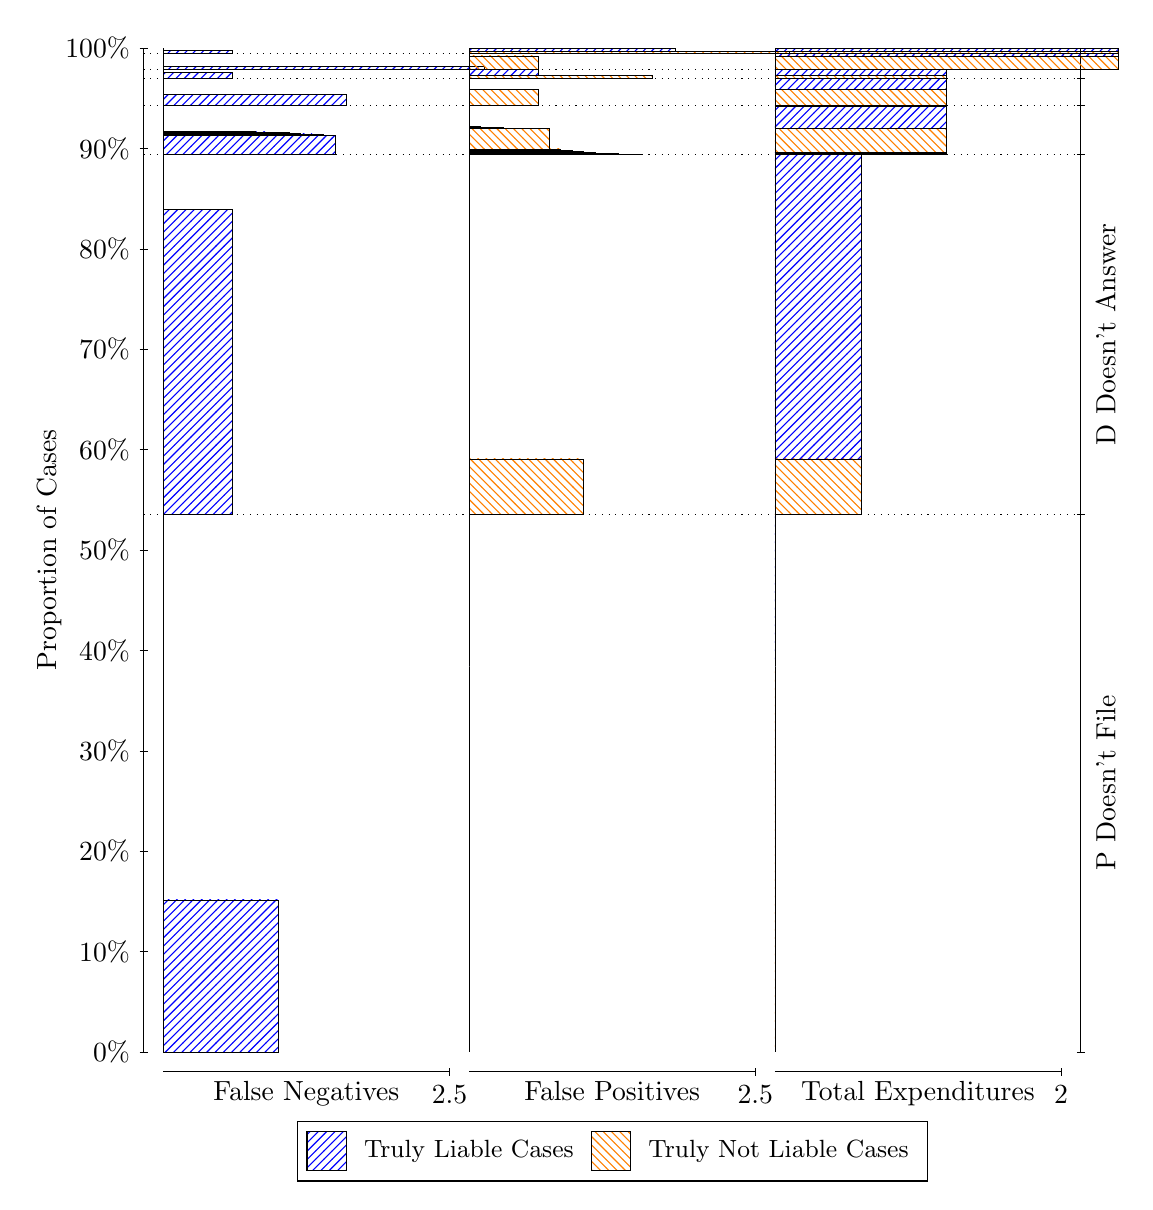
\begin{tikzpicture}
\draw[black, very thin] (1.5,1.75) -- (1.5,14.5);
\node[rotate=90, text=black, anchor=center] at (0.3, 8.125) {Proportion of Cases};
\draw[black, very thin] (1.45,1.75) -- (1.55,1.75);
\node[text=black, anchor=east] at (1.45, 1.75) {0\%};
\draw[black, very thin] (1.45,3.025) -- (1.55,3.025);
\node[text=black, anchor=east] at (1.45, 3.025) {10\%};
\draw[black, very thin] (1.45,4.3) -- (1.55,4.3);
\node[text=black, anchor=east] at (1.45, 4.3) {20\%};
\draw[black, very thin] (1.45,5.575) -- (1.55,5.575);
\node[text=black, anchor=east] at (1.45, 5.575) {30\%};
\draw[black, very thin] (1.45,6.85) -- (1.55,6.85);
\node[text=black, anchor=east] at (1.45, 6.85) {40\%};
\draw[black, very thin] (1.45,8.125) -- (1.55,8.125);
\node[text=black, anchor=east] at (1.45, 8.125) {50\%};
\draw[black, very thin] (1.45,9.4) -- (1.55,9.4);
\node[text=black, anchor=east] at (1.45, 9.4) {60\%};
\draw[black, very thin] (1.45,10.675) -- (1.55,10.675);
\node[text=black, anchor=east] at (1.45, 10.675) {70\%};
\draw[black, very thin] (1.45,11.95) -- (1.55,11.95);
\node[text=black, anchor=east] at (1.45, 11.95) {80\%};
\draw[black, very thin] (1.45,13.225) -- (1.55,13.225);
\node[text=black, anchor=east] at (1.45, 13.225) {90\%};
\draw[black, very thin] (1.45,14.5) -- (1.55,14.5);
\node[text=black, anchor=east] at (1.45, 14.5) {100\%};

\draw[black, very thin] (13.4,1.75) -- (13.4,14.5);
\draw[black, very thin] (13.35,1.75) -- (13.45,1.75);
\node[anchor=west] at (13.35, 1.75) {};
\draw[black, very thin] (13.35,8.5799) -- (13.45,8.5799);
\node[anchor=west] at (13.35, 8.5799) {};
\draw[black, very thin] (13.35,13.148) -- (13.45,13.148);
\node[anchor=west] at (13.35, 13.148) {};
\draw[black, very thin] (13.35,13.771) -- (13.45,13.771);
\node[anchor=west] at (13.35, 13.771) {};
\draw[black, very thin] (13.35,14.11) -- (13.45,14.11);
\node[anchor=west] at (13.35, 14.11) {};
\draw[black, very thin] (13.35,14.231) -- (13.45,14.231);
\node[anchor=west] at (13.35, 14.231) {};
\draw[black, very thin] (13.35,14.431) -- (13.45,14.431);
\node[anchor=west] at (13.35, 14.431) {};
\draw[black, very thin] (13.35,14.5) -- (13.45,14.5);
\node[anchor=west] at (13.35, 14.5) {};

\draw[black, very thin, pattern color=blue, pattern=north east lines] (1.75,1.75) rectangle (3.2033,3.6816);
\draw[black, very thin, pattern color=orange, pattern=north west lines] (1.75,3.6816) rectangle (1.75,8.5799);
\draw[black, very thin, pattern color=blue, pattern=north east lines] (1.75,8.5799) rectangle (2.622,12.446);
\draw[black, very thin, pattern color=orange, pattern=north west lines] (1.75,12.446) rectangle (1.75,13.148);
\draw[black, very thin, pattern color=blue, pattern=north east lines] (1.75,13.148) rectangle (3.93,13.393);
\draw[black, very thin, pattern color=blue, pattern=north east lines] (1.75,13.393) rectangle (3.7847,13.403);
\draw[black, very thin, pattern color=blue, pattern=north east lines] (1.75,13.403) rectangle (3.6393,13.411);
\draw[black, very thin, pattern color=blue, pattern=north east lines] (1.75,13.411) rectangle (3.494,13.418);
\draw[black, very thin, pattern color=blue, pattern=north east lines] (1.75,13.418) rectangle (3.3487,13.428);
\draw[black, very thin, pattern color=blue, pattern=north east lines] (1.75,13.428) rectangle (3.2033,13.431);
\draw[black, very thin, pattern color=blue, pattern=north east lines] (1.75,13.431) rectangle (3.058,13.436);
\draw[black, very thin, pattern color=blue, pattern=north east lines] (1.75,13.436) rectangle (2.9127,13.438);
\draw[black, very thin, pattern color=blue, pattern=north east lines] (1.75,13.438) rectangle (2.7673,13.439);
\draw[black, very thin, pattern color=orange, pattern=north west lines] (1.75,13.439) rectangle (1.75,13.771);
\draw[black, very thin, pattern color=blue, pattern=north east lines] (1.75,13.771) rectangle (4.0753,13.912);
\draw[black, very thin, pattern color=orange, pattern=north west lines] (1.75,13.912) rectangle (1.75,14.11);
\draw[black, very thin, pattern color=blue, pattern=north east lines] (1.75,14.11) rectangle (2.622,14.186);
\draw[black, very thin, pattern color=orange, pattern=north west lines] (1.75,14.186) rectangle (1.75,14.231);
\draw[black, very thin, pattern color=blue, pattern=north east lines] (1.75,14.231) rectangle (5.8193,14.262);
\draw[black, very thin, pattern color=orange, pattern=north west lines] (1.75,14.262) rectangle (1.75,14.431);
\draw[black, very thin, pattern color=blue, pattern=north east lines] (1.75,14.431) rectangle (2.622,14.47);
\draw[black, very thin, pattern color=orange, pattern=north west lines] (1.75,14.47) rectangle (1.75,14.5);
\draw[black, very thin, pattern color=orange, pattern=north west lines] (5.6333,1.75) rectangle (5.6333,6.6483);
\draw[black, very thin, pattern color=blue, pattern=north east lines] (5.6333,6.6483) rectangle (5.6333,8.5799);
\draw[black, very thin, pattern color=orange, pattern=north west lines] (5.6333,8.5799) rectangle (7.0867,9.2822);
\draw[black, very thin, pattern color=blue, pattern=north east lines] (5.6333,9.2822) rectangle (5.6333,13.148);
\draw[black, very thin, pattern color=orange, pattern=north west lines] (5.6333,13.148) rectangle (7.8133,13.15);
\draw[black, very thin, pattern color=orange, pattern=north west lines] (5.6333,13.15) rectangle (7.668,13.153);
\draw[black, very thin, pattern color=orange, pattern=north west lines] (5.6333,13.153) rectangle (7.5227,13.159);
\draw[black, very thin, pattern color=orange, pattern=north west lines] (5.6333,13.159) rectangle (7.3773,13.164);
\draw[black, very thin, pattern color=orange, pattern=north west lines] (5.6333,13.164) rectangle (7.232,13.177);
\draw[black, very thin, pattern color=orange, pattern=north west lines] (5.6333,13.177) rectangle (7.0867,13.186);
\draw[black, very thin, pattern color=orange, pattern=north west lines] (5.6333,13.186) rectangle (6.9413,13.201);
\draw[black, very thin, pattern color=orange, pattern=north west lines] (5.6333,13.201) rectangle (6.796,13.218);
\draw[black, very thin, pattern color=orange, pattern=north west lines] (5.6333,13.218) rectangle (6.6507,13.48);
\draw[black, very thin, pattern color=blue, pattern=north east lines] (5.6333,13.48) rectangle (6.36,13.481);
\draw[black, very thin, pattern color=blue, pattern=north east lines] (5.6333,13.481) rectangle (6.2147,13.484);
\draw[black, very thin, pattern color=blue, pattern=north east lines] (5.6333,13.484) rectangle (6.0693,13.489);
\draw[black, very thin, pattern color=blue, pattern=north east lines] (5.6333,13.489) rectangle (5.924,13.492);
\draw[black, very thin, pattern color=blue, pattern=north east lines] (5.6333,13.492) rectangle (5.7787,13.502);
\draw[black, very thin, pattern color=blue, pattern=north east lines] (5.6333,13.502) rectangle (5.6333,13.771);
\draw[black, very thin, pattern color=orange, pattern=north west lines] (5.6333,13.771) rectangle (6.5053,13.97);
\draw[black, very thin, pattern color=blue, pattern=north east lines] (5.6333,13.97) rectangle (5.6333,14.11);
\draw[black, very thin, pattern color=orange, pattern=north west lines] (5.6333,14.11) rectangle (7.9587,14.156);
\draw[black, very thin, pattern color=blue, pattern=north east lines] (5.6333,14.156) rectangle (6.5053,14.231);
\draw[black, very thin, pattern color=orange, pattern=north west lines] (5.6333,14.231) rectangle (6.5053,14.4);
\draw[black, very thin, pattern color=blue, pattern=north east lines] (5.6333,14.4) rectangle (5.6333,14.431);
\draw[black, very thin, pattern color=orange, pattern=north west lines] (5.6333,14.431) rectangle (9.7027,14.46);
\draw[black, very thin, pattern color=blue, pattern=north east lines] (5.6333,14.46) rectangle (8.2493,14.5);
\draw[black, very thin, pattern color=orange, pattern=north west lines] (9.5167,1.75) rectangle (9.5167,6.6483);
\draw[black, very thin, pattern color=blue, pattern=north east lines] (9.5167,6.6483) rectangle (9.5167,8.5799);
\draw[black, very thin, pattern color=orange, pattern=north west lines] (9.5167,8.5799) rectangle (10.607,9.2822);
\draw[black, very thin, pattern color=blue, pattern=north east lines] (9.5167,9.2822) rectangle (10.607,13.148);
\draw[black, very thin, pattern color=orange, pattern=north west lines] (9.5167,13.148) rectangle (11.697,13.161);
\draw[black, very thin, pattern color=blue, pattern=north east lines] (9.5167,13.161) rectangle (11.697,13.17);
\draw[black, very thin, pattern color=orange, pattern=north west lines] (9.5167,13.17) rectangle (11.697,13.481);
\draw[black, very thin, pattern color=blue, pattern=north east lines] (9.5167,13.481) rectangle (11.697,13.755);
\draw[black, very thin, pattern color=orange, pattern=north west lines] (9.5167,13.755) rectangle (11.697,13.764);
\draw[black, very thin, pattern color=blue, pattern=north east lines] (9.5167,13.764) rectangle (11.697,13.771);
\draw[black, very thin, pattern color=orange, pattern=north west lines] (9.5167,13.771) rectangle (11.697,13.97);
\draw[black, very thin, pattern color=blue, pattern=north east lines] (9.5167,13.97) rectangle (11.697,14.11);
\draw[black, very thin, pattern color=orange, pattern=north west lines] (9.5167,14.11) rectangle (11.697,14.156);
\draw[black, very thin, pattern color=blue, pattern=north east lines] (9.5167,14.156) rectangle (11.697,14.231);
\draw[black, very thin, pattern color=orange, pattern=north west lines] (9.5167,14.231) rectangle (13.877,14.4);
\draw[black, very thin, pattern color=blue, pattern=north east lines] (9.5167,14.4) rectangle (13.877,14.431);
\draw[black, very thin, pattern color=orange, pattern=north west lines] (9.5167,14.431) rectangle (13.877,14.46);
\draw[black, very thin, pattern color=blue, pattern=north east lines] (9.5167,14.46) rectangle (13.877,14.5);
\draw[black, dotted] (1.5,8.5799) -- (13.4,8.5799);
\draw[black, dotted] (1.5,13.148) -- (13.4,13.148);
\draw[black, dotted] (1.5,13.771) -- (13.4,13.771);
\draw[black, dotted] (1.5,14.11) -- (13.4,14.11);
\draw[black, dotted] (1.5,14.231) -- (13.4,14.231);
\draw[black, dotted] (1.5,14.431) -- (13.4,14.431);
\draw[black, very thin] (1.75,1.5) -- (5.3833,1.5);
\node[text=black, anchor=north] at (3.5667, 1.5) {False Negatives};
\draw[black, very thin] (5.3833,1.45) -- (5.3833,1.55);
\node[text=black, anchor=north] at (5.3833, 1.45) {2.5};

\draw[black, very thin] (5.6333,1.5) -- (9.2667,1.5);
\node[text=black, anchor=north] at (7.45, 1.5) {False Positives};
\draw[black, very thin] (9.2667,1.45) -- (9.2667,1.55);
\node[text=black, anchor=north] at (9.2667, 1.45) {2.5};

\draw[black, very thin] (9.5167,1.5) -- (13.15,1.5);
\node[text=black, anchor=north] at (11.333, 1.5) {Total Expenditures};
\draw[black, very thin] (13.15,1.45) -- (13.15,1.55);
\node[text=black, anchor=north] at (13.15, 1.45) {2};

\node[text=black, centered, rotate=90] at (13.72, 5.165) {P Doesn't File};
\node[text=black, centered, rotate=90] at (13.72, 10.864) {D Doesn't Answer};






\draw (7.449999999999999,1.5) node[draw=none] (baseCoordinate) {};
\begin{scope}[align=center]
        \matrix[scale=0.5, draw=black, below=0.5cm of baseCoordinate, nodes={draw}, column sep=0.1cm]{
            \node[rectangle, draw, minimum width=0.5cm, minimum height=0.5cm, pattern color=blue, pattern=north east lines] {}; &
            \node[draw=none, font=\small, text=black] (B) {Truly Liable Cases}; &
            \node[rectangle, draw, minimum width=0.5cm, minimum height=0.5cm, pattern color=orange, pattern=north west lines] {}; &
            \node[draw=none, font=\small, text=black] (B) {Truly Not Liable Cases}; \\
            };
\end{scope}

\end{tikzpicture}
\end{document}